\documentclass[12pt, a4paper]{article} 
\usepackage{eurosym}  
\usepackage[margin = 1.2in]{geometry}
\usepackage[french]{babel}
\usepackage[utf8x]{inputenc}
\usepackage{graphicx}
\usepackage[T1]{fontenc}
\usepackage{fancyhdr}
\usepackage{hyperref}
\usepackage{listings}
\usepackage{setspace}
\pagestyle{fancy}
\setlength{\headheight}{15pt}
\fancyhead[L]{SharpBoy}
\fancyhead[R]{EPITA}
\fancyhead[C]{S\_Society}
\renewcommand{\footrulewidth}{1pt} 
\fancyfoot[L]{Rapport de projet}
\fancyfoot[R]{2017}
\fancyfoot[C]{\thepage}
\title{\Huge \bf SharpBoy}
\author{\large \bf S\_Society }
\title{\large \bf Rapport de Projet}

\begin{document}



\maketitle


\bigskip
\large Gabriel DUQUE: duque\_g

\bigskip
\large Antoine MARTIN: ma\_9

\bigskip
\large Martin MEUNIER : meunie\_o

\bigskip
\large Ilyes NOUMRI : noumri\_i

\bigskip
\large {\textbf{Projet S2\#}}

\bigskip 
\bigskip
\bigskip


\begin{center}

\includegraphics[width= 12cm]{logo-epita-hd.png} 
\end{center}

\pagebreak

\tableofcontents 

\linespread{1.4}
\pagebreak

\lstset{language=Caml}

\pagebreak

\large
\section{Retour sur le cahier des charges}
\large



\subsection{Introduction}
Voici notre rapport final, contenant de nombreuses informations sur le déroulement de notre projet de sa conception à sa réalisation et détaillant de nombreux points techniques de notre émulateur. Il reprend des éléments des deux rapports précédents de manière plus détaillée et ajoute de nouvelles informations sur la progression effectuée entre la deuxième et troisième soutenance. 

\begin{center}
\includegraphics[width = 10.4 cm]{Game-Boy-FL.png}
\end{center}

\pagebreak
\subsection{Équipe}
L'équipe n'a pas changé et est toujours aussi motivé pour mener le projet à bien. Elle est constituée de Gabriel DUQUE, Antoine MARTIN, Martin MEUNIER, Ilyes NOUMRI.
\bigskip

Notre équipe s'est formée assez rapidement dans le sens où Ilyes, Antoine et moi-même étions devenus très bons amis pendant le S1\# et il nous a donc semblé naturel de se mettre ensembles pour le projet de S2\#.
\bigskip

Par la suite, Martin nous a vite montré son intérêt concernant le projet et est donc devenu le quatrième membre de notre groupe \textit{s-society}.

\bigskip
Le nom de notre groupe: s-society est issu d'une série télévisée nommée \textit{Mr. Robot} où le personnage principale est membre d'un groupe nommé 'f-society'. Dans notre cas, s-society signifie 'sharp society', un jeu de mot entre le nom de notre classe et un l'adjectif anglais 'sharp' pouvant signifier vif d'esprit.
\pagebreak

\subsubsection{Gabriel DUQUE (duque\_g) :}
Depuis toujours, je suis un grand passionné des ordinateurs. Je suis un très grand fan de Linux et de l'Open Source en général. Après un an et demi en médecine, j'ai eu l'occasion de me réorienter et aller à EPITA. 
\bigskip

Je ne suis pas un grand amateur de jeu vidéo, c'est pourquoi, bien qu'il ait un rapport avec les jeux vidéo, j'ai autant apprécié réaliser un projet assez complexe, tant au niveau théorique qu'au niveau pratique. La seule console à laquelle j'ai beaucoup joué a été la GameBoy et c'est pour ça que j'étais très content de pouvoir en émulateur.
\bigskip

Je suis ravi d'avoir eu la chance de pouvoir réaliser un tel projet en première année. Les connaissances que j'ai acquises et le temps que j'ai passé à coder n'a fait que confirmer le fait que je ne m'épanouissait pas en médecine et que j'étais plutôt fait pour l'informatique. Je pense avoir forgé de très bons liens avec mes camarades.
\bigskip

En plus d'avoir pu apprendre beaucoup de chose en informatique, en tant que chef de groupe je pense avoir mûri et appris beaucoup de choses concernant la gestion d'un projet et des différents profils lors d'un travail de groupe.
\pagebreak


\subsubsection{Antoine MARTIN (ma\_9) :}

\bigskip
Je suis intéressé par les ordinateurs depuis que je suis petit. Après une tentative ratée au concours de médecine, j'ai changé de direction pour étudier l'informatique qui a toujours été un hobby. 

J'ai donc rejoint EPITA par la rentrée décalée, en même temps que Gabriel, qui vient du même amphithéâtre de médecine que moi.

\bigskip
Je suis passionné par Linux, l'Open Source et à peu près tout ce qui implique un ordinateur.

\bigskip
Ce projet est principalement un moyen d'en apprendre plus sur l'émulation et sur l'architecture de la GameBoy.

J'ai découvert les émulateurs il y a longtemps et me suis toujours demandé comment ils fonctionnaient. Je me rends compte maintenant qu'en apprendre sur les émulateurs c'est aussi en apprendre beaucoup sur les ordinateurs qu'ils imitent, et que c'est un sujet extrêmement intéressant impliquant de multiples disciplines enseignées à l'EPITA.

\bigskip
Outre l'intérêt pour l'émulation, c'est aussi l'attrait d'un nouveau langage, le F\#, qui me motive dans ce projet.

\bigskip
Enfin, je pense en avoir appris beaucoup sur le travail de groupe et/ou personnel durant ce projet.

\pagebreak
\subsubsection{Martin MEUNIER (meunie\_o) :}

\bigskip
Ayant rejoint EPITA en 2015 et ayant refais mon S1, je repars avec de meilleures bases dans toutes les matières. Nous nous sommes retrouvés avec mes amis pour ce projet s’annonçant palpitant ! 

\bigskip
J’ai toujours aimé les anciennes consoles car nous avons tous grandis avec quelques une comme la Gameboy et nous allons maintenant coder notre premier émulateur. C’est une fierté pour moi de faire ce projet d’émulateur et je suis, comme mes amis, super motivé pour le mener à bout. Le fonctionnement des CPU est très intéressant et nous avons tous voulus y prêter attention. J’espère que ce projet m’apportera d’énormes connaissances pour la suite de ma scolarité à EPITA. 

\bigskip
De plus, le fait de faire du F\# m’intéresse vraiment et cela donne l’impression d’un vrai challenge de projet. J’espère que ce projet vous plaira autant qu’il nous a plu.

\bigskip
C'était mon point de vue du début du projet. Aujourd'hui, nous avons achevé le projet. Nous sommes fiers de notre travail et je suis personnellement contenant de ce qu'est j'ai appris tout au long du projet.

\bigskip
J'ai aujourd'hui 20 ans et c'est avec joie que nous vous présentons notre Sharpboy. Après quelques mois de travail intense, autant sur la Chip-8 que sur l'émulation de la GameBoy, nos deux émulateurs ont atteints nos principaux objectifs. 

\pagebreak
\subsubsection{Ilyes  NOUMRI (noumri\_i) :}
\medskip

Depuis que je suis petit, je joue sur PC à différents émulateurs et notamment des émulateurs de GameBoy. C’est pourquoi, l’idée de développer un émulateur de GameBoy m’a vraiment emballé !
\medskip

Je suis aussi intéressé par le fonctionnement des processeurs et des ordinateurs en général. J’ai rencontré Antoine et Gabriel l’année dernière en classe de Sharp et ayant de nombreux points communs nous sommes devenus rapidement amis. 
\medskip

J’ai connu Martin de mon année de S1 car il était dans ma classe et il a vite rejoint l’équipe . Le projet pourrait nous apporter plein de connaissances sur le fonctionnement des CPUs qui pourraient nous être utiles personnellement et pour le reste de nos études.

\bigskip
Le projet étant fini, mes espérances quant à ce que le projet pourrait m'apporter se sont produites. J'ai en effet appris beaucoup quant au fonctionnement d'un processeur et d'un système mais aussi quant au travail d'équipe et à l'importance de la communication. 

\pagebreak
\bigskip
\subsection{Le contexte historique}
Nintendo est une marque japonaise de divertissement vidéoludique née en 1889. Originellement, Nintendo était une marque de jeu proposant comme produit phare des cartes de jeu japonais, les \textit{hanafudas}. Par la suite, vers la fin des années 1940, la marque décide de se diversifier en proposant des produits et services variés, allant des portions de riz individuelles à la gestion de compagnies de taxi en passant par l'ouverture de love hotels au Japon.

En 1959, le vent tourne pour la firme japonaise grâce à un contrat signé avec Disney qui lui permet de se positionner sur la scène internationale. La compagnie rentre finalement en bourse en 1962 sous le nom de Nintendo Co. Ltd. 

Au cours des années 70, la marque se rend bien compte du potentiel que représente le marché naissant du jeu vidéo et décide de s'atteler à le conquérir. Nintendo commence par construire des jeux pour les bornes d'arcade, profitant de leur expansion massive. En collaboration avec Magnavox, Nintendo participe à la production de l'Odyssey, la première console de salon multi-jeux en 1972.

\pagebreak
\bigskip
\subsection{Répartition des tâches}
\bigskip

La répartition des tâches n'a pas changé même si elle reste approximative pour la SharpBoy sachant que nous avançons beaucoup en groupe.

\bigskip
\bigskip
\begin{center}
\begin{tabular}{|l|c|c|c|c|}
\hline
\bf Tâches                & \bf Gabriel   & \bf Antoine   & \bf Martin    & \bf Ilyes\\
\hline 
Menus/Options       &      x       &               &         x     &       \\
\hline 
Site web            &               &         x     &               &     x  \\
\hline 
Vidéo               &          x    &               &       x       &       \\
\hline 
CPU                 & x             & x             &               &       \\
\hline 
Mémoire             &               & x             &               &  x \\
\hline
Audio               &               &               & x             & x \\
\hline
Marketing           & x             &               &               & x \\
\hline
Réseau              &               &               & x             & x \\ 
\hline
\end{tabular}
\end{center}
\bigskip
\pagebreak

\subsection{Nos débuts}

Au début de notre travail de projet, nous voulions nous informer  sur les principes de l'émulation. 

\bigskip
Nous avons réalisé un émulateur de Chip 8 car nous avions besoin d'avoir une première expérience en émulation. Selon de nombreux blogs spécialisés dans le sujet, il était conseillé de commencer par ce genre d'émulateur pour comprendre leur structure générale.



\bigskip
Ensuite, nous nous sommes lancés sur l'élaboration de l'émulation de la GameBoy. Après plusieurs semaines de recherches et de lecture, nous nous sommes beaucoup renseignés sur le fonctionnement intégral et l'élaboration de la GameBoy.

\bigskip
Enfin, à la deuxième soutenance, nous avons présenté le début de notre émulateur où nous avons montré le jeu TETRIS complètement fonctionnel.

\pagebreak
\subsection{Notre émulateur Chip 8}
Lors de la première soutenance, nous avions présenté un émulateur de Chip 8 fonctionnel. Celui-ci nous a permit d'avoir une solide base de connaissances pour l'émulateur de GameBoy.

Par ailleurs, puisque nous avions décidé de développer notre émulateur en F\#, le développement de la Chip 8 nous a permit d'améliorer nos compétences dans ce langage.



\subsection{Notre émulateur de GameBoy: SharpBoy}

Lors de la deuxième soutenance nous avons présenté un émulateur fonctionnel, capable de charger plusieurs jeux basiques.

SharpBoy ne gère pas du tout les sorties audio ; nous avons choisi de concentrer notre travail sur autre chose car le son est une des parties les plus complexes de l'émulation et il n'est pas essentiel pour la majorité des jeux.
\medskip

Pour cette troisième soutenance, nous nous sommes concentrés sur la gestion de jeux plus complexes, afin d'étendre grandement le catalogue de jeux jouables sur SharpBoy.

\subsection{GitHub }

Nous avons toujours notre dépôt GitHub à disposition nous permettant de travailler efficacement en groupe et de répertorier tout notre travail.Notre organisation GitHub \textit{s-society} a deux dépôts GitHub, le premier pour l'émulateur de Chip 8 et le deuxième, SharpBoy pour notre émulateur de GameBoy.

Nous avons bloqué les ajouts sur la branche principale de notre dépôt pour nous forcer à lire le code des autres avant de l'intégrer à la branche principale pour vérifier l'exactitude du code, et que tout le monde le comprenne dans son entièreté.Le fruit de cette méthode a été une progression commune des membres de l'équipe.

De plus, grâce au "pull request" de GitHub, un semblant de liste de choses à faire s'est naturellement créé au début du projet. Par la suite, nous nous sommes chacun attelé petit à petit à la tâche. Aussi, le fait de réduire les fonctions compliquées en un assemblage de fonctions élémentaires a rendu la tâche plus aisée et nous a donné l'impression de vraiment progresser dans notre projet

\subsection{Un site Web}

Notre site Web : \url{http://sharpboy.xyz}

Ce site contient un lien vers la dernière version de notre émulateur et l'avancement de notre projet. Nous avons automatisé l'ajout d'une section commentaires à chaque article du site.

\bigskip
\subsection{Planning}

\bigskip

\begin{center}
\begin{tabular}{|l|c|c|c|}
\hline
\bf Tâches          & \bf Soutenance 2      & \bf Soutenance 3  \\
\hline 
Menus/Options       &        20\%           & 100\%  \\
\hline 
Site web            &        100\%         & 100\%  \\
\hline 
Vidéo               &        100\%          & 100\%  \\
\hline 
CPU                 &        66\%          & 100\%  \\
\hline 
Mémoire             &        66\%         & 100\%  \\
\hline
Audio               &        0\%           & 100\%  \\
\hline
Réseau              &        0\%           & 100\%  \\

\hline
\end{tabular}
\end{center}
\bigskip
Ce planning n'a au final pas été extrêmement précis, puisqu'il a été écrit au tout début du projet, alors que nous n'avions aucune idée de la manière dont notre travail allait évoluer. 

La réalité a été assez différente de ce tableau : En terme de menus et options, nous ne proposons au final qu'un dialogue de chargement de fichier au lancement de l'émulateur afin de sélectionner la ROM désirée.
L'audio n'était finalement pas réalisable, et les fonctionnalités réseau n'ont pas vu le jour non plus.

Nous sommes tout de même fiers du travail accompli, les catégories restantes étant assez conséquentes (Mémoire, CPU, Vidéo).

La prévision du gros des tâches du projet est certainement un point à améliorer pour nos travaux futurs.
\pagebreak

\subsection{Problèmes rencontrés pendant le projet}

Depuis le début du projet, nous avons rencontrés quelques soucis tout au long de la conception et l'élaboration de nos deux émulateurs.

\bigskip
En effet, lors de l'élaboration de notre Chip 8 nous avions eu des problèmes lors des phases de tests de ROMs où certains jeux ne fonctionnaient pas et nous avions dû déboguer notre émulateur pour trouver les problèmes. Finalement, notre émulateur de Chip 8 fonctionnait avec toutes nos ROMs.

\bigskip
Pour notre émulateur de GameBoy, SharpBoy, nous avons tout de suite vu la difficulté d'optimisation pour tous les types de ROMs existants. Il existe en effet environ 6 types de cartouches, chacune ayant une manière différente de se charger en mémoire. 

Pour faire face à ce problème, nous avons dans un premier temps décidé de ne nous occuper que du premier type de cartouche, se chargeant en mémoire directement (les autres types sont découpés en plusieurs secteurs) pour prouver que notre émulateur fonctionnait correctement. 

\bigskip
Nous avons étudié avec précision toute la documentation de l'émulation de la GameBoy qui n'était pas facile à comprendre mais que nous avons tous apprivoisée avec le temps pour être prêts sur le sujet. De plus, le son est aussi auxiliaire et nous poserait trop de problèmes à l'heure actuelle pour que nous nous en occupions.
\pagebreak

\bigskip
La dernière difficulté majeure rencontrée durant ce projet est le problème de la complexité du programme avec lequel nous travaillions : une fois devant un problème, les possibilités d'origine sont multiples. Un problème d'affichage par exemple, peut provenir d'une erreur dans la fonction d'affichage elle même, ou bien être dû à une erreur dans la gestion de l'adressage mémoire, ou encore dans le traitement de la logique pure de la ROM. 

\bigskip
Cet empilement de plusieurs éléments interdépendants a rendu les problèmes inexpliqués difficiles à régler.

\subsection{Avancement du projet}

Depuis la deuxième soutenance, nous avons implémenté le support pour des cartouches plus évoluées, utilisant des contrôleurs de banque mémoire (MBCs). Ce sont des puces intégrées aux cartouches, qui gèrent elles même l'adressage dans la cartouche. Il a donc fallu gérer les différents cas de figure incluant ces puces.


\pagebreak
\section{Partie Technique}
\subsection{Introduction}

Après avoir vu en détail comment notre projet s'était déroulé d'un point de vue humain nous allons maintenant vous présenter la GameBoy d'un point de vue plus technique.

Cette partie du rapport de projet a pour but de donner quelques précisions techniques concernant notre progression et notre conception des problèmes algorithmiques que nous avons rencontrés.

Pour comprendre la documentation ci-après il est important de comprendre que l''élément essentiel de la GameBoy est le CPU qui exécute les commandes contenues dans le cartouche du jeu (la ROM). 

Concrètement, chaque problème et chaque séquence de code est divisée en un certain nombre d'instructions élémentaires appelés "opcodes" par calque sur le terme anglais. Ces opcodes sont au nombre d'environ 500 (en comptant les opcodes ayant un "préfixe" changeant leur signification) et s'écrivent par paire de deux caractères hexadécimaux (de 0 à F).
\pagebreak

\subsection{Spécifications techniques}

La Chip 8 fut un excellent sujet d'étude afin de se familiariser avec un appareil à la structure en comparaison simple, tout en amenant suffisamment de challenge pour nous en apprendre beaucoup durant notre travail sur celle ci.

\bigskip
Le Chip 8 n'était pas un appareil physique à proprement parler, il s'agissait en fait d'une machine purement virtuelle, destinée à être émulée, pour faciliter la programmation de jeux simples.

\bigskip
\bigskip
\begin{center}
\begin{tabular}{|l|c|}
\hline
\bf Élément          & \bf Informations \\
\hline
RAM & 4kB\\
\hline 
Son & Juste un bip possible\\
\hline
Écran & 64 * 32\\
\hline
Couleurs & Monochrome, pas de nuances\\
\hline
\end{tabular}
\end{center}

\bigskip
\bigskip
\pagebreak
En comparaison, la GameBoy est donc beaucoup plus puissante, et possède une architecture plus complexe.

Voici un tableau récapitulatif des différents éléments de la GameBoy ainsi que quelques cartouches de base. 

\bigskip
\begin{center}
\begin{tabular}{|l|c|}
\hline
\bf Élément          & \bf Informations \\
\hline
CPU & Architecture 8-bit semblable au Z80 à 4,2 MHz\\
\hline
Bus de donnée & 8 bits\\
\hline
Bus d'adresse & 16 bits\\
\hline
RAM principale & 8kB\\
\hline
RAM graphique & 8kB\\
\hline 
Son & 4 canaux stéréo\\
\hline
Écran & 160 * 144\\
\hline
Couleurs & 4 nuances de gris\\
\hline
\end{tabular}
\end{center}

\bigskip
Les cartouches de GameBoy peuvent avoir une ROM de 256kb, 512kb, 1Mb, 2Mb, 4Mb ou 8Mb au maximum. Elles peuvent également contenir d'autres éléments, comme des extensions de RAM ou même des puces utilisée pour une partie des calculs. C'est la présence de ces différents éléments supplémentaires qui détermine le type de cartouche.

\pagebreak
\subsection{Les registres}

\subsubsection{Généralités}

Les registres représentent la mémoire interne du processeur. Ils sont de petite taille, généralement 8 ou 16 bits et sont la mémoire la plus rapide d'un ordinateur. Les registres permettent de stocker les données nécessaires à l'exécution des instructions.

Dans la Chip 8, ceux ci sont au nombre de 16, allant de V0 à VF (numérotation hexadécimale), et peuvent stocker chacun 8 bits. En plus de ceux si, elle en possède 3 particuliers, le registre d'adresses I ainsi que PC et SP, détaillés plus bas.

Le processeur de la GameBoy est similaire aux processeurs Intel 8080 et Zilog Z80. Il possède huit registres de 8 bits: A, B, C, D, E, F, H et L, et deux registres de 16 bits: SP et PC.

De plus, certaines instructions permettent de traiter une paire de registres de 8 bits comme un unique registre de 16 bits en les associant. Les paires possibles pour ces registres combinés sont: AF, BC, DE et HL.

\pagebreak
\bigskip
\bigskip
\small \begin{lstlisting}[frame=single]
let mutable A = 0x01uy
let mutable B = 0uy
let mutable C = 0x13uy
let mutable D = 0uy
let mutable E = 0xD8uy
let mutable F = 0b10110000uy
let mutable H = 0x01uy
let mutable L = 0x4Duy
let mutable SP = 0xFFFEus
let mutable PC = 0x0100us
\end{lstlisting}
\bigskip
\bigskip
\large

Vous pouvez voir ci-dessus leur déclaration en F\# en tant que "mutables" ce qui leur permet de changer de valeur au cours de l'exécution du programme. Vous remarquerez qu'ils ne sont pas tous initialisés à 0.

Les registres sont ainsi utilisés pour contenir les variables et portions de code (appelées sous-routines) nécessaires à l'exécution du programme. 


La majorité des instructions ont donc pour fonction de manipuler la mémoire dans les registres à travers de nombreuses actions simples comme par exemple l'incrémentation d'un registre ou la comparaison de deux valeurs situées dans des registres.

\pagebreak

Au sein de ces registres, certains ont un usage général et d'autres ont un rôle particulier nécessaire au bon fonctionnement de la machine. Nous allons maintenant détailler le fonctionnement de trois d'entre eux ainsi que ce qu'ils représentent.

\subsubsection{Les registres particuliers}

Parmi les registres que nous allons détailler les caractéristiques ici, deux sont de seize bits, PC et SP et un est de huit bits, F.

\bigskip
\begin{center}{\bf Program Counter :}\end{center}
Premièrement, le registre PC est sûrement le plus simple à comprendre. En effet, ce registre de 16 bits a simplement pour but de pointer vers la prochaine instruction à exécuter dans la mémoire de la GameBoy d'où son nom "Program Counter". 

Il est commun à la GameBoy et à la Chip 8, c'est en effet un élément clé de l'exécution du programme.

\bigskip

Ce registre est initialisé à \$100 et c'est ainsi l'instruction stockée à cet endroit dans la mémoire qui est exécutée au démarrage de la console. Par la suite, ce registre va être manipulé (la plupart du temps incrémenté pour passer à l'instruction suivante) de manière indirecte par les opcodes eux-même qui exécutent une action puis, par exemple, incrémentent PC pour passer à l'instruction suivante.

\pagebreak
\bigskip
\begin{center}{\bf Stack Pointer :}\end{center}
Deuxièmement, le registre SP ("Stack Pointer") est un peu plus compliqué à comprendre que le précédent. Cela étant dit, sa compréhension est tellement importante lors de l'émulation d'un processeur qu'il est impossible de passer à côté de sa signification. De plus bien assimiler le mode de fonctionnement de SP permet de comprendre aussi comment l'assembleur est utilisé. Il est également présent et dans la GameBoy et dans la Chip 8.

\bigskip

La première chose à savoir est que la GameBoy stocke toutes les variables, arguments des sous-routines, adresses de retour (...) dans une pile ("stack" en anglais). le Stack Pointer pointe vers le haut de la pile. 

Il faut savoir que le pile grandit vers le bas "dans les adresses mémoire" ce qui signifie que la pile commence à la dernière adresse mémoire de la mémoire concernée. 

\bigskip

Par exemple, pour la RAM interne basse de la GameBoy qui s'étend de \$C000 à \$DFFF il faut initialiser SP à \$EOOO et non à \$BFFF (On l'initialise à \$E000 et non \$DFFF car SP se décrémente tout seul avant d'ajouter un élément à la pile). 

Encore une fois, en comparaison le Stack Pointer de la Chip 8 est plus simple, SP étant simplement incrémenté de 0x0 à 0xF et la pile ne pouvant contenir que 16 valeurs au maximum.

\pagebreak
Cela étant dit, bien que la majorité des programmeurs initialisent SP autre part, la GameBoy initialise SP d'elle-même à \$FFFE (En haut de la RAM de la console).

\bigskip

Par la suite, plusieurs opcodes permettent de faire grandir la pile ou au contraire de la réduire. Pour en augmenter la taille, CALL, PUSH et RST sont disponibles et pour la réduire, POP, RET et RETI.

\bigskip


\begin{center}{\bf Le registre "flag"}\end{center}

Sur la Chip 8, le registre VF est particulier : il n'est pas conseillé aux programmeurs de stocker des valeurs importantes dedans, celui ci étant utilisé par la machine pour signaler des situations particulières : dans le cas d'un under/overflow, par exemple, ce registre stocke une valeur de 1 au lieu de 0 pour indiquer la situation qui vient de se produire.

\bigskip
On retrouve ce concept dans la GameBoy, en bien plus élaboré, le registre F contenant en fait plusieurs bits indiquant chacun une situation particulière.

Le registre "flag" signifiant drapeau en anglais a donc pour utilité comme son nom l'indique de signaler une situation. Un tableau représentant ce registre de 8 bits sera plus adapté pour les explications car visualiser ce registre rend sa compréhension aisée.
\pagebreak
\bigskip
\bigskip
\bigskip
\begin{center}
\begin{tabular}{|l|c|c|c|c|c|c|c|}
\hline
7 & 6 & 5 & 4 & 3 & 2 & 1 & 0 \\
\hline
\bf Z & \bf N & \bf H & \bf C & \bf 0 &  \bf 0 & \bf 0 & \bf 0 \\
\hline
\end{tabular}
\end{center}
\bigskip


Les quatre bits de poids faible numérotés de 0 à 3 sont initialisés à 0 et ne changent jamais. Ils n'ont pas non plus de signification particulière.

Les quatre bits de poids forts sont par définition à 0 ou à 1. Chacun de ces bits est utilisé de manière booléenne pour indiquer l'occurrence d'une situation particulière lors d'un calcul.

\bigskip
Le bit Z (le bit de poids le plus fort) est initialisé à 1 sert à indiquer que le résultat d'une opération mathématique est égal à 0 ou alors que la comparaison de deux valeurs avec l'instruction \textit{CP} était positive. Son utilité est principalement d'éviter de faire des opérations impossibles en mathématiques, notamment la division par 0.
\bigskip

Le bit N est initialisé à 0 et indique si une soustraction a eu lieu lors de la dernière instruction. Les nombres négatifs étant représentés par des bits signés en informatique, il est essentiel de savoir si une soustraction a eu lieu car le résultat de cette soustraction peut être négatif et sera donc traité de manière différente.
\bigskip

\pagebreak

Avant de vous détailler les bits H et C, il est important de savoir ce que signifie le mot anglais "carry". Ce mot peut être traduit par retenue dans le domaine dont nous parlons. 

\bigskip
Par exemple, si on se place sur un registre de huit bits qui a pour valeur \%11111111 (255 en décimal) et qu'on lui ajoute 1, en théorie, on obtient \%100000000 (256 en décimal). Cependant, étant sur des registres de huit bits, il est impossible d'écrire les neufs bits. Le bit de poids le plus fort, le seul à être à 1 sera perdu et le registre prendra la valeur \%00000000. Évidemment, cela est problématique car 255 + 1 = 256 et non 0. La retenue est appelée "carry".
\bigskip


Le bit H est mis à 1 s'il y a eu un "half-carry" ce qui signifie un "carry" sur les 4 bits de poids le plus faible par exemple il y a "half-carry" dans l'opération \%00001111 + \%00000001 = \%00010000 . Il est initialisé à 1.
\bigskip

Le bit C est mis à 1 s'il y a eu un "carry" sur les huit bits du registre courant, comme par exemple dans l'opération donnée dans l'explication du terme "carry". Ce bit est également initialisé à 1.



\subsection{Le chargement des ROMs}

S'agissant de la Chip 8, le chargement des ROMs était assez direct : On copiait juste l'intégralité de la ROM dans la mémoire vive de la Chip 8, à partir de l'adresse 0x200 (les adresses avant celle ci étant réservées au stockage des polices d'écriture).
\pagebreak

\bigskip
Pour la GameBoy, ce mode de fonctionnement existe aussi, cependant il existe très peu de jeux utilisant ce mode. La plupart des cartouches contiennent en fait en plus de la mémoire contenant le jeu, du matériel supplémentaire.
\bigskip
Il existe plusieurs types de cartouches pour la GameBoy. Celles-ci ont été créées dans le but de répondre au besoin des éditeurs et développeurs, pour créer des jeux plus complexes et plus complet pour la console. Les cartouches sont différenciées par leur façon de gérer la mémoire à travers une puce appelée Memory Bank Controller. 

\bigskip
Elles permettent d'éviter la limitation de 16 bits d'adresse de la GameBoy. Elles permettent aussi de sélectionner les banques de mémoire de la RAM et de la ROM assignées à la GameBoy ainsi d'activer, désactiver la RAM supplémentaire de la cartouche (si elle en possède une) et des éléments matériels de la cartouche (si disponible aussi).

\bigskip

Les adresses de la mémoire allant de \$0000-\$7FFF à \$A000-\$BFFF peuvent être utilisé pour lire et écrire sur la cartouche. 

\bigskip

Pour déterminer le type de cartouche, on regarde à l'adresse mémoire \$0147 de la ROM dans laquelle est spécifié une valeur correspondant à un type de cartouche.

\bigskip
\pagebreak
\bigskip
Voici les différentes valeurs possibles :

\bigskip
\bigskip
\bigskip

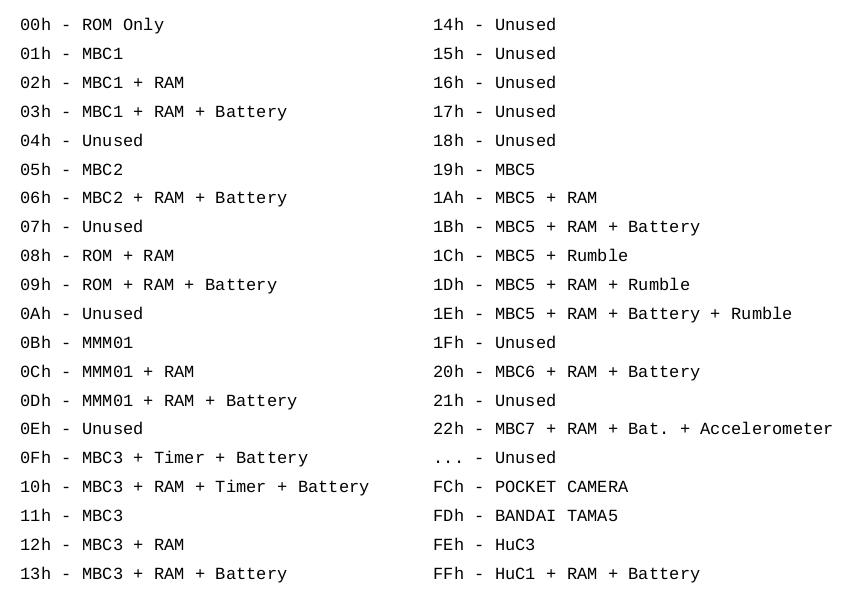
\includegraphics[width = 14.5 cm]{MBCtype.png}





\bigskip
\pagebreak

\subsubsection{Les différents types de MBC}

Si la ROM n'a pas besoin de MBC, elle peut écrire sur toute la mémoire allouée à la lecture et écriture sur la cartouche sans restrictions. 

\begin{center}
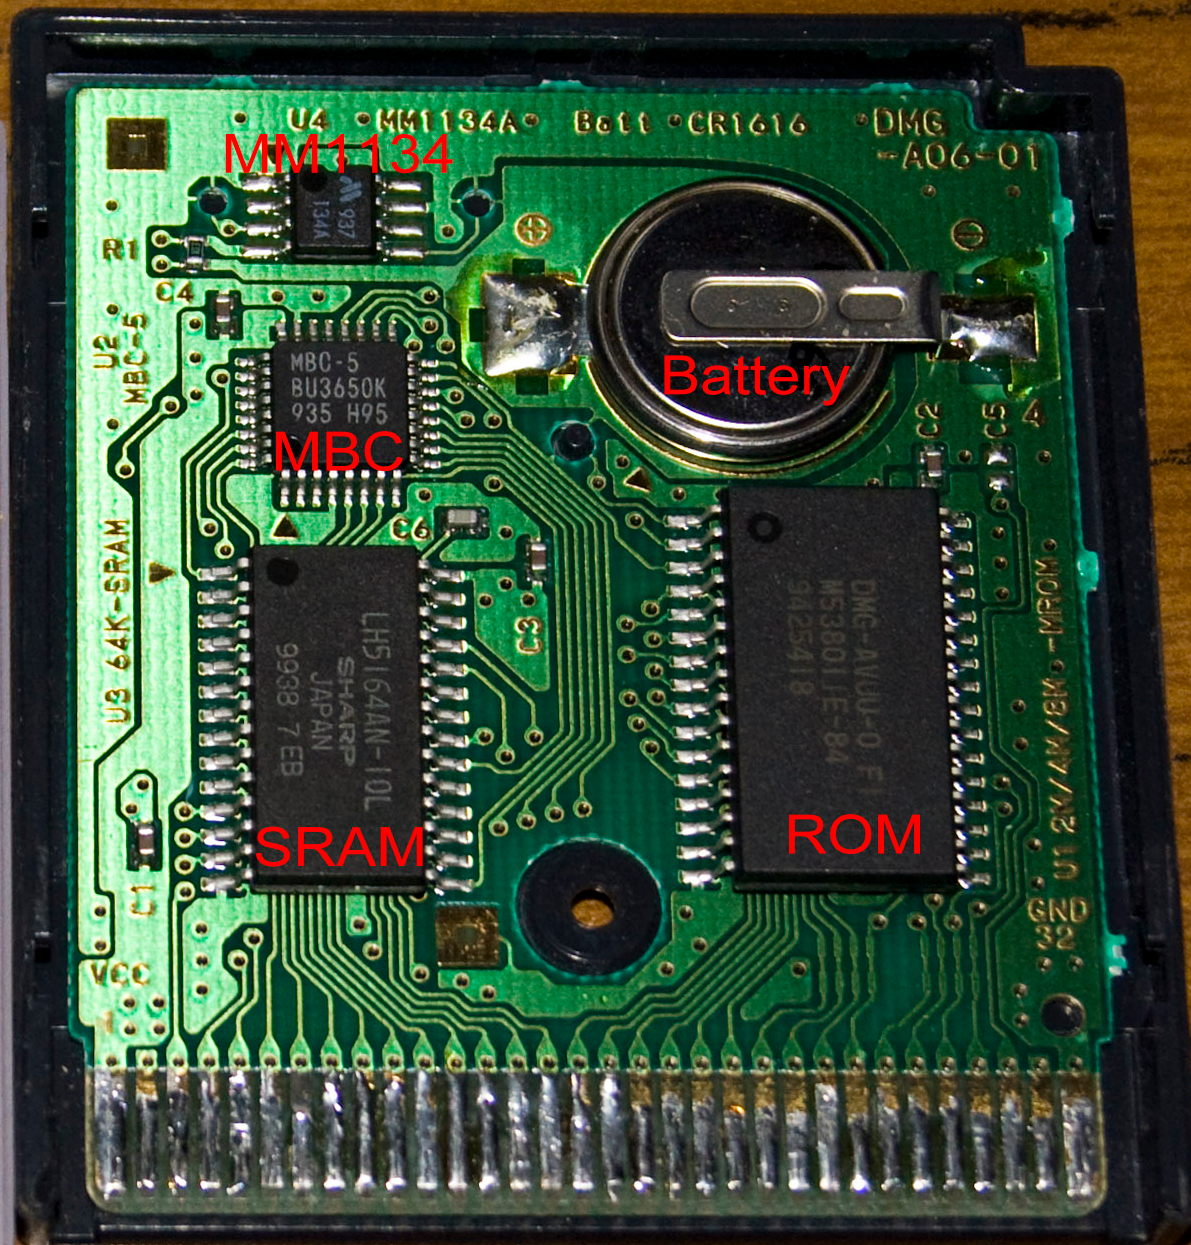
\includegraphics[width = 10.4 cm]{MBCinside.jpg}
\end{center}

Sinon, elle a différentes propriétés selon le type de cartouches :

\bigskip

- MBC 1 : La ROM peut avoir une taille maximum de 2 MB et intégrer une RAM de 32KB.

\bigskip

- MBC 2 : La ROM peut avoir une taille maximum de 256KB et intégrer une RAM de 2KB.

\bigskip

- MBC 3 : La ROM peut avoir une taille maximum de 2 MB et intégrer une RAM 64 KB.


\bigskip

(Il n'y a pas de MBC 4.)

\bigskip

- MBC 5 :  Elles sont utilisées par les roms de GameBoy Color principalement et peuvent avoir une taille maximum de 8 MB jusqu'à 128KB de RAM.

\bigskip

\begin{center}{\bf MBC1}\end{center}
\bigskip



Nous avons choisi choisi d'implémenter le type MBC1 pour plusieurs raisons. Premièrement, nous avons choisi le MBC1 parce qu'il s'agit de la première MBC à avoir vu le jour. Ensuite, nous sommes tous les quatre de grands amateurs de \textit{La Légende de Zelda} et les cartouches de GameBoy du premier opus de la saga sont de type MBC1.
\bigskip

Les cartouches "ROM only"\footnote{Sans MBC} ont deux banques de ROM qui s'étendent de \$0000 à \$3FFF pour ROM0 et de \$4000 à \$7FFF pour ROM1. Ainsi, ces cartouches n'ont que 32 kB de ROM. ROM0 représente le coeur du jeu en lui-même, les opcodes qui gèrent les données du jeu alors que ROM1 contient plutôt les données de l'utilisateur.
\bigskip

Le but des cartouches MBC1 est d'augmenter la quantité disponible de ROM et de RAM dans la cartouche. En effet, les MBCs sont l'avancée qui a permis à la GameBoy de dominer le marché de la console portable (qu'elle a créé en soit puisqu'il s'agit de la première console portable).
\bigskip

\pagebreak
La ROM (Read Only Memory) est donc divisée en plusieurs banques de 16kB chacune. Le moyen que les programmeurs ont trouvé pour sélectionner l'une ou l'autre de ces banques est le suivant: le MBC (lorsqu'il est là évidemment) intercepte les bits envoyés sur la plage \$2000 - \$3FFF en écriture et cela lui permet de choisir une ROM de 16kB à charger sur la plage qu'occupe exclusivement ROM1 dans le cas où il n'y a pas de MBC, \$4000 - \$7FFF.  
\bigskip

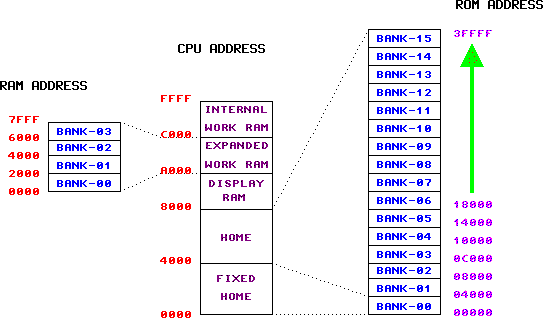
\includegraphics[width = 15 cm]{memory1.png}
\bigskip



Ce qu'il se passe en réalité: l'opcode envoie une suite d'instructions permettant d'écrire un entier sur 5 bits dans une adresse de la plage \$2000 - \$3FFF (5 dans l'adresse \$2000 dans l'argument suivant). Avant qu'elle ne soit exécutée (elle ne pourrait pas l'être parce qu'on n'écrit pas sur la ROM), elle est interprétée par le MBC comme une instruction de 'charger' la banque ROM numérotée par le nombre qui était censé être écrit dans la ROM. 
\bigskip

\bigskip
\small{\begin{lstlisting}[frame=single]
LD	A,5
LD	HL,\$2000
LD	(HL),A
\end{lstlisting}}
\bigskip
\large

Dans l'exemple précédent, le résultat est le chargement de la banque ROM5 dans la plage \$4000 - \$7FFF. Le nombre s'écrivant sur cinq bits, il peut y avoir $2^5$ banques de ROM différentes. Ce concept décrit le premier mode de fonctionnement du MBC1: le mode 16Mbit ROM/ 8KByte RAM (externe).
\bigskip

En parallèle, une autre configuration du MBC1 permet d'augmenter la RAM plutôt que la ROM. D'une manière analogue, tenter d'écrire un nombre sur  deux bits sur la plage \$4000 - \$5FFF aboutira au chargement d'une banque de RAM numérotée avec le nombre écrit sur 2 bits.
\bigskip

Ainsi, cette deuxième utilisation permet d'avoir potentiellement quatre banques de RAM plutôt qu'une. Sachez néanmoins que ces modes ne sont pas mutuellement exclusifs et une cartouche MBC1 peut très bien varier entre les modes pour permettre de répondre à ses besoins.
\bigskip

Finalement, bien que nous ne les ayions pas implémentés, les autres types de cartouches ne marchent pas exactement selon le même principe mais il s'agit de découpes différentes de mémoire et le processus est très similaire.
\bigskip


\pagebreak
\subsection{Le processeur de la GameBoy}

Le GameBoy utilise un micro-processeur similaire à un Intel 8080. Il contient toutes les instructions d'un 8080, sauf qu'il n'y a pas d'instructions d'échange. Pourtant, le processeur est plus similaire au processeur Zilog Z80. Comparé au Z80, quelques instructions ont été ajoutées et certaines ont été enlevées.
\bigskip

Nous n'allons pas lister toutes les instructions ajoutées ou enlevées mais nous pouvons dire que certaines instruction ADD et LD ont été ajoutés et que certaines instructions IN/OUT par exemple ont été enlevés.

\begin{center}
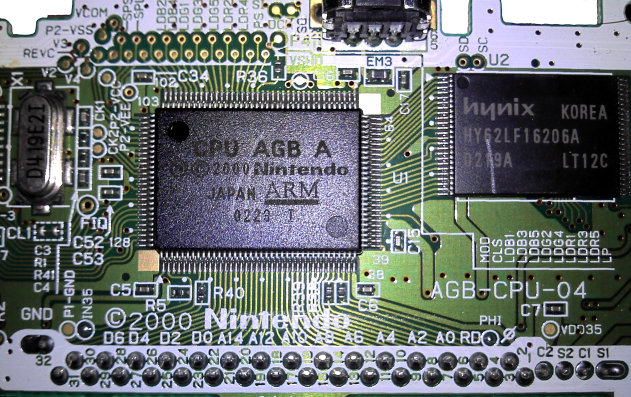
\includegraphics[width = 15 cm]{proc.png} 
\end{center}

\pagebreak

\subsection{La fonction principale}

Le code source contenu dans le fichier Program.fs est le maître d'orchestre de tout l'émulateur. En effet, il est le fichier général qui va appeler les fonctions des autres fichiers pour pouvoir lancer les ROMs et faire avancer l'émulateur dans celle-ci. C'est aussi dans ce fichier que sont gérées les interruptions du programme.
\bigskip



Le fichier Program.fs peut être découpé en plusieurs parties distinctes qui ont chacune une fonction bien définie dans le processus de l'émulation.
\bigskip


Le première chose faite lors du lancement de l'émulateur est l'ouverture d'un dialogue avec l'utilisateur pour que celui ci sélectionne la ROM. Grâce aux bibliothèques Windows.Forms cette tâche a été plutôt aisée. Nous nous sommes alors rendu compte qu'un des avantages majeurs du F\# était de donner la possibilité au programmeur de combiner un langage fonctionnel puissant avec le "framework" .NET développé par Microsoft.
\bigskip
\small{\begin{lstlisting}[frame=single]
let openRomDialog = new OpenFileDialog()
    openRomDialog.Title <-"Select Game Boy ROM" 
    openRomDialog.Filter <-"Gameboy ROM Files|*.gb|All files|*.*"
\end{lstlisting}}
\bigskip
\large
Par la suite, la ROM est chargée en mémoire et certains bits sont lus pour pouvoir obtenir des informations concernant la ROM comme par exemple sont type (ROM only, MBC1, MBC1 avec extension de RAM ...) ou alors son origine\footnote{Nous avons négligé ce genre d'informations car elles ne portent que peu d'intérêt pour jouer} (Japonaise ou alors étrangère).
\bigskip
\pagebreak
\small{\begin{lstlisting}[frame=single]
if openRomDialog.ShowDialog() = DialogResult.OK then
        Memory.rom <- File.ReadAllBytes(openRomDialog.FileName)
    else Environment.Exit(1)

    if rom.Length > int (snd ROM1+1us) then
        rom.[0..int (snd ROM1)].CopyTo(memory,0)
    else
        rom.CopyTo(memory,0)
\end{lstlisting}}
\bigskip
\large
La ROM chargée, le contenu de l'adresse \$0147 est lu et défini le type de cartouche. Cette étape est cruciale au fonctionnement de l'émulateur car elle définit comment le contenu sera écrit dans la mémoire et comment on y accédera par la suite.
\bigskip
\tiny{\begin{lstlisting}[frame=single]
Memory.cartridge <- LanguagePrimitives.EnumOfValue<byte, 
                    Memory.Cartridge>(memory.[0x0147])
    
Memory.mbcType <- match cartridge with
                  | Memory.Cartridge.Mbc1 
                  | Memory.Cartridge.Mbc1Ram 
                  | Memory.Cartridge.Mbc1RamBatt -> Memory.Mbc.Mbc1
                  | Memory.Cartridge.Mbc2 
                  | Memory.Cartridge.Mbc2Batt -> Memory.Mbc.Mbc2
                  | Memory.Cartridge.Mbc3 
                  | Memory.Cartridge.Mbc3Ram 
                  | Memory.Cartridge.Mbc3RamBatt 
                  | Memory.Cartridge.Mbc3TimerBatt 
                  | Memory.Cartridge.Mbc3TimerRamBatt -> Memory.Mbc.Mbc3
                  | _ -> Memory.Mbc.RomOnly
\end{lstlisting}}
\large
\bigskip
Pour pouvoir commencer à traiter les opcodes, il faut implémenter les périphériques de sortie notamment pour l'affichage. Un certain nombre de variables sont déclarées à ce moment là pour pouvoir être ensuite utilisées par les fonctions qui suivent.  

\small{\begin{lstlisting}[frame=single]
 let SCREEN_WIDTH = 160 
    let SCREEN_HEIGHT = 144
    let SCALE = 2

let screenBuffer = Array.create (SCREEN_WIDTH*SCREEN_HEIGHT) 0
\end{lstlisting}}
\bigskip
\large

\pagebreak

Les fonctions utilisées uniquement dans le Program.fs sont ensuite définies et seulement certaines d'entre celles-ci seront détaillées plus loin dans cette documentation. D'une manière générale, ces fonctions gèrent l'affichage à travers la construction de sprites et les interruptions de l'émulateur pour attendre une action de l'utilisateur.
\bigskip

Toutes les variables et fonctions étant maintenant définies, les pièces du puzzle commencent finalement par s'assembler dans la boucle principale qui permet à la mécanique du jeu d'avancer de manière cyclique.

\small{\begin{lstlisting}[frame=single]
let Loop  =
        async {
        while true do
            if not stopped then
                // Un tour de la boucle //
        }
\end{lstlisting}}
\bigskip
\large

Vous pouvez voir que cette structure simpliste de la boucle permet de bien visualiser le squelette du fonctionnement de la GameBoy. En outre le mot-clé \textit{async} permet au programme de continuer à avancer et donc de répondre aux commandes de l'utilisateur lorsque la boucle tourne.  

\bigskip
L'intérieur de la boucle a la structure suivante:la lecture de l'opcode, l'exécution de l'opcode puis la gestion des conséquences de l'opcode en lui-même s'il y en a (Affichage d'un sprite, interruption du programme si certains "flags" sont mis à 1 due à l'opcode exécuté.). 

\pagebreak
\subsection{Sortie Vidéo}

Le contrôleur vidéo de la GameBoy peut afficher jusqu'à 40 sprites soit en 8x8 ou en 8x16 pixels (tous de la même taille). En raison d'une limitation du matériel, seuls dix sprites peuvent être affichés par ligne de balayage. 
\bigskip

La GameBoy peut aussi afficher un fond d'écran, ainsi qu'une fenêtre (deuxième fond superposé au premier et n'occupant pas forcément tout l'écran).

Le registre situé à l'adresse \$FF40, LCDC (LCD Controler) stock 8 bits contenant la majeure partie de la configuration de l'affichage.

\bigskip
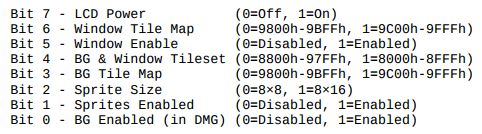
\includegraphics[width=12cm]{display.png}
\bigskip

On peut voir ici que ce registre permet d'activer/désactiver les sprites ou le background, de passer du mode 8x8 au mode 8x16, ainsi que de sélectionner la partie de la mémoire utilisée pour stocker la disposition du fond d'écran et de la fenêtre.

\bigskip
Ce fond d'écran fait 256x256 pixels, ce qui permet de le faire défiler sur l'écran, qui ne fait que 160x144 pixels. Le fond est composé de 32x32 tuiles, de 8x8 pixels chacune. Cette organisation en tuile permet de réutiliser ces tuiles pour construire un niveau.
\pagebreak

\bigskip
Pour les éléments mobiles de l'affichage, on utilise les sprites. Les schémas des sprites sont stockés sous le même format que les tuiles, mais sont stockés dans un endroit différent de la mémoire.

\bigskip
Si des sprites avec des coordonnées différentes se superposent, celui avec la plus petite coordonnée X aura la priorité sur les autres et apparaîtra au dessus.

Si des sprites avec les mêmes coordonnées X se superposent, le sprite avec l'emplacement mémoire le plus petit est prioritaire.

\bigskip
Pour cacher des sprites hors de l'écran, on leur assigne les coordonnées X=0 et Y=0. Pour les afficher dans le coin en haut à gauche on utilise les coordonnées X=8, Y=16. Il faut donc tenir compte de ce décalage pour l'affichage.

\bigskip
Seulement 10 sprites peuvent être affiché sur une ligne horizontale ; les sprites non utilisés sont donc en général cachés en mettant leur coordonnée Y à 0, la coordonnée X à 0 pouvant les positionner hors de l'écran sans pour autant les empêcher d'affecter les autres sprites sur la même ligne.

\bigskip
Enfin, chaque sprite possède des attributs stockés dans 4 octets:

\bigskip
\begin{itemize}
    \item 0 : position Y
    \item 1 : position X
    \item 2 : numéro de la disposition du sprite (parmis les 255 dispositions stockées)
\end{itemize}

\bigskip
\pagebreak
L'octet numéro 3 possède 8 bits, dont les 4 de poids fort stockent une information sur le sprite :

\bigskip
\begin{itemize}
    \item 7 : Priorité. Si ce bit est à 0 le sprite apparaît au dessus de la fenêtre et du fond. S'il est à 1 ce sprite ne prévaut que sur la couleur 0 du fond et de la fenêtre.
    \item 6 : Renversement vertical. Si ce bit est à 1 ce sprite est inversé selon l'axe vertical
    \item 5 : Renversement horizontal. Si ce bit est à 1 ce sprite est inversé selon l'axe horizontal.
    \item 4 : Numéro de palette. Sélectionne parmi les deux palettes de nuances de gris en fonction de ce bit.  
\end{itemize}



\pagebreak

\subsection{Instruction DAA : Traduction binaire/décimal}

L'instruction DAA (Decimal Adjust register A) permet de convertir le contenu du registre A en code BCD (binary coded decimal).

\bigskip
Cette fonction est essentielle, elle permet en effet de traduire tous les chiffres que la ROM veut afficher du binaire vers le décimal, permettant un affichage lisible "humainement" pour l'utilisateur.

\bigskip

\small{\begin{lstlisting}[frame=single]
let daa () =
    let lowBCD = A % 10uy
    let highBCD = ((A % 100uy) - lowBCD) / 10uy
    let result = (highBCD <<< 4) ||| lowBCD
    ZF <- (result = 0uy)
    HF <- false
    CF <- A >= 100uy
    A <- result
\end{lstlisting}}

\bigskip
\large

Note : l'ajout de parenthèses vides après le nom de la fonction dans la déclaration permet au compilateur de la distinguer d'une variable, et donc de ne pas l'évaluer lorsqu'elle est déclarée mais lorsqu'elle sera appelée.

\bigskip
La fonction, une fois son but effectué, modifie plusieurs flags du registre F pour indiquer le résultat de l'opération.

\pagebreak
\subsection{La fonction Draw}
\small \begin{lstlisting}[frame=single]
let Draw (args:PaintEventArgs) =
  for y in [0..HEIGHT-1] do
    for x in [0..WIDTH-1] do
      args.Graphics.FillRectangle(brushes.[screen.[(y*WIDTH) + x]],
      x * SCALE, y * SCALE, SCALE, SCALE)
\end{lstlisting}
\large
La fonction Draw est une fonction utilisant System.Drawing et Windows.Form qui permet de dessiner sur l'écran de la GameBoy grâce à deux boucles permettant de parcourir tout l'écran. La fonction dessine grâce à FillRectangle qui reçois les coordonnées du rectangle à remplir.

\bigskip

\subsection{Exemple de fonctions d'incrémentations}
\small { \begin{lstlisting}[frame = single]
let inc (reg:byte byref) =
     reg <- reg + 1uy
     ZF <- (reg = 0uy) 
     NF <- false
     HF <- (reg = 0xF0uy)
     
let incHL () =
    temp <- readAddress_2(H,L)
    inc(&temp) 
    writeAddress_2(H,L,temp)

let incrementHL(inc:bool) =
     temp16 <- uint16 H <<< 8 ||| uint16 L 
     (if inc then temp16 <- temp16 + 1us 
             else temp16 <- temp16 - 1us)
     H <- byte ((temp16 &&& 0xFF00us) >>> 8) 
     L <- byte (temp16 &&& 0x00FFus)
\end{lstlisting}} 
\bigskip

\pagebreak
\large
La fonction inc permet d'incrémenter la variable contenue dans les registre donné en argument, ainsi que définir la valeur des flags ZF, NF et HF. 
Les fonctions incHL et incrementHL sont utilisées dans des instructions.
incHL permet d'incrémenter la valeur dans l' adresse du registre HL . Le mot clé \& indique que l'on veut passer une variable par référence. incrementHL, quant à elle, permet d'incrémenter l'adresse du registre HL si le booléen est à true sinon il la décrémentera.


De la même manière, la fonction dec :

\bigskip
\begin{lstlisting}[frame=single]
let dec (reg:byte byref) =
     reg <- reg - 1uy
     ZF <- (reg = 0uy) 
     NF <- true
     HF <- (reg = 0x0Fuy)
\end{lstlisting}

\pagebreak
\subsection{Fonctions booléennes}

L'émulateur utilise beaucoup de fonctions permettant de comparer des bits entre eux, comme ces deux fonctions OR et XOR

\bigskip
\small\begin{lstlisting}[frame=single]
let orA (n:byte) =
     A <- A ||| n 
     ZF <- (A = 0uy) 
     NF <- false
     HF <- false
     CF <- false 

let xorA (n:byte) =
     A <- A ^^^ n 
     ZF <- (A = 0uy) 
     NF <- false
     HF <- false
     CF <- false
\end{lstlisting}
\large

Ces fonctions s'appliquent au registre A, et appliquent l'opération de manipulation de bits OR ou XOR sur A et l'octet passé en argument \textit{n}.

\pagebreak

\subsection{Exemples d'opcodes}

\small{ \begin{lstlisting}[frame = single]

opcode.[0x04] <- (fun () -> inc(&B); PC <- PC + 1us; 1uy)


opcode.[0x27] <- (fun () -> daa (); PC <- PC + 1us; 1uy)
\end{lstlisting}}
\bigskip
\large

Voici quelques exemples d'opcodes :

\bigskip

- L'opcode correspondant à l'adresse 0x04 utilise la fonction  d'incrémentation (vu plus haut) pour incrémenter  le registre B et augmenter le compteur.

\bigskip

- L'opcode correspondant à l'adresse 0x27 utilise la fonction de traduction binaire/décimal vu au-dessus puis passe à l'instruction suivante.


\pagebreak
\section{Récit de la réalisation}

Nous avons commencé avec la Chip 8, ce qui nous a permis de comprendre les principes fondamentaux de l'émulation, qui sont nécessaires pour programmer la Chip 8 ; l'avantage de celle ci étant qu'elle ne présente pas d'autre challenge supplémentaire : se concentrer sur l'acquisition des connaissances sur l'émulation était déjà une difficulté en soit, nous n'avions pas besoin de problèmes techniques supplémentaires.

\bigskip
Une fois notre baptême de l'émulation effectué, nous pouvions nous lancer dans la GameBoy, qui représente une complexité accrue par rapport à la Chip 8, dans tous ses aspects. 

\bigskip
La première étape était d'obtenir une sortie vidéo : en effet, sans celle ci, difficile de juger de la bonne exécution de nos jeux sur l'émulateur. Une fois un rendu basique obtenu, nous avons pu déboguer nos jeux petit à petit, assez pour pouvoir présenter un émulateur fonctionnel à la deuxième soutenance. 

\bigskip
Cependant il était loin d'être complet : de nombreuses fonctionnalités manquaient encore et il était clair que nous ne pourrions pas toutes les implémenter. Nous avons donc décidé d'étendre sa compatibilité avec les jeux, au détriment du son et d'autres fonctionnalités comme la sauvegarde ou l'émulation du câble multijoueur.

\bigskip
Nous avons fait ce choix car notre émulateur manquait cruellement de choix de jeux : sans implémenter les contrôleurs de banque mémoire, moins d'une dizaine de jeux connus étaient jouables.


\pagebreak

\section{Exemples de jeux testés}

\subsection{TETRIS}

\subsubsection{Informations}
Date de parution : 1989

Type de cartouche : ROM Only

Développé par : Nintendo

\bigskip
\begin{center}
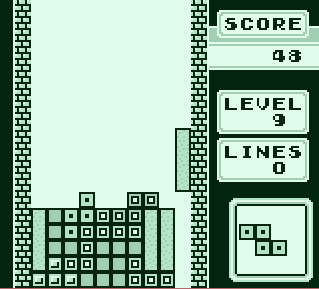
\includegraphics[width=11cm]{Capture3.PNG}
\end{center}

\bigskip
\subsubsection{Problèmes rencontrés}
Nous avons eu des problèmes sur ce jeu au niveau de l'optimisation avant la deuxième soutenance, mais après celle-ci, ce jeu fonctionnait parfaitement sans aucun bug.

\bigskip
Nous n'avons donc pas de problèmes actuellement pour cette ROM.



\pagebreak
\subsection{Dr Mario}

\subsubsection{Informations}

Date de parution :1990

Type de cartouche : ROM Only

Développé par : Nintendo

\bigskip
\begin{center}
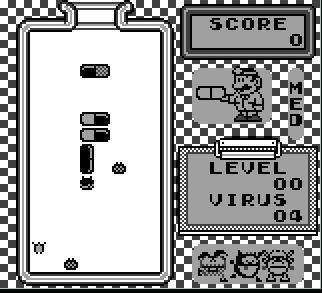
\includegraphics[width=11cm]{drmario.jpg}
\end{center}

\subsubsection{Problèmes rencontrés}
Ce jeu fonctionne parfaitement depuis la seconde soutenance, nous n'avons donc pas de problème aujourd'hui.

\pagebreak
\subsection{The Legend of Zelda: Link's Awakening}

\subsubsection{Informations}
Date de parution :1993

Type de cartouche : MBC1

Développé par : Nintendo

\bigskip
\begin{center}
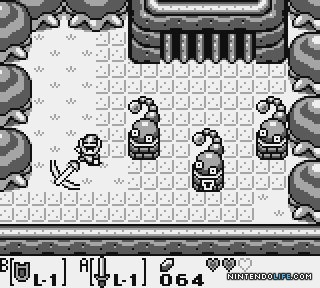
\includegraphics[width=11cm]{zelda.jpg}
\end{center}

\bigskip
\subsubsection{Problèmes rencontrés}
Pour ce jeu, nous avons rencontrés quelques problèmes. Tout d'abord, les sprites du jeu sont buggés, c'est à dire que visuellement le jeu n'est pas entièrement déchiffrable. De plus, il existe des conflits causant des crashs de l'émulateur lorsque nous tuons tout les ennemis d'une pièce par exemple. Sans aucune raison, les trois sauvegardes du jeu censées être vides nous emmènent à un endroit différent du jeu. Le jeu n'est donc pas jouable mais la ROM se lance correctement comme prévu.

\pagebreak

\subsection{AlleyWay}

\subsubsection{Informations}

Date de parution :1989

Type de cartouche : ROM Only

Développé par : Nintendo

\bigskip
\begin{center}
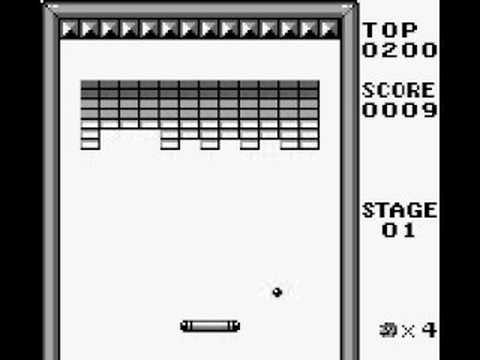
\includegraphics[width=11cm]{alleyway.jpg}
\end{center}

\subsubsection{Problèmes rencontrés}
Ce jeu fonctionne parfaitement depuis la seconde soutenance, nous n'avons donc pas de problème aujourd'hui.

\pagebreak
\subsection{Astérix}

\subsubsection{Informations}
Date de parution :1993

Type de cartouche : MBC

Développé par : Bit Managers

\bigskip
\begin{center}
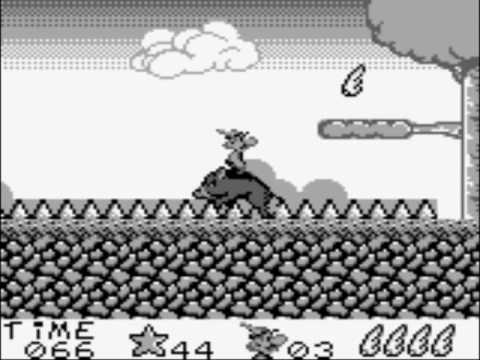
\includegraphics[width=11cm]{asterix.jpg}
\end{center}

\bigskip
\subsubsection{Problèmes rencontrés}

Dans ce jeu vidéo, toutes les mécaniques de jeu fonctionnent correctement : Asterix peut sauter, donner des coups de poing aux romains et au sanglier, sauter sur les plateformes.

Le seul problème du jeu est la disposition de certains sprites dans le jeu : cela crée des zones de différentes hauteurs qui se réajustent au fil du jeu mais cela peut créer des conflits comme tomber au mauvais endroit et mal se positionner dans une zone particulière du jeu.

\pagebreak
\subsection{Aladdin}

\subsubsection{Informations}

Date de parution :1993

Type de cartouche : MBC

Développé par : Virgin Interactive

\bigskip
\begin{center}
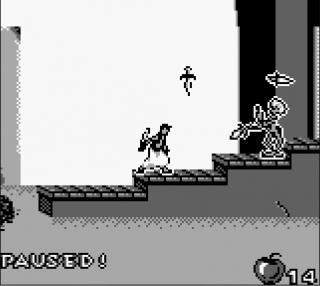
\includegraphics[width=11cm]{aladdinGB.jpg}
\end{center}

\subsubsection{Problèmes rencontrés}
Dans ce jeu vidéo, toutes les mécaniques de jeu fonctionnent bien : Nous pouvons sauter et lancer des bombes aux ennemis. Les ennemis meurent bien et les interactions avec le décor fonctionnent (nous pouvons par exemple sauter sur le chameau au début du jeu ).

Un des problèmes apparaissant fréquemment est un crash du jeu au bout d'un certain temps de jeu.



\pagebreak

\subsection{Batman Forever}

\subsubsection{Informations}
Date de parution : 1995

Type de cartouche : MBC

Développé par : Acclaim Entertainment

\bigskip
\begin{center}
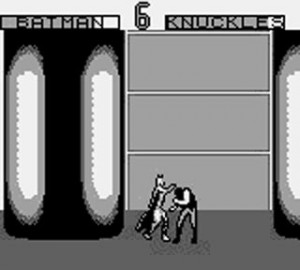
\includegraphics[width=11cm]{batman.jpg}
\end{center}
\bigskip
\subsubsection{Problèmes rencontrés}

Nous pouvons jouer à ce jeu vidéo correctement : nous pouvons sélectionner nos armes au début du stage et ensuite lancer la partie et commencer à battre les ennemis qui arrivent avec nos coups de pied ! De plus les interactions avec le décor fonctionnent bien, nous pouvons nous cacher correctement.

\bigskip
Le problème central de cette cartouche est un problème d'affichage (de sprite) qui rend invisible certaines parties du corps de Batman et des ennemis. On retrouve ce problème d'affichage dans les menus, lors de la sélection des armes par exemple.

\pagebreak

\section{Conclusion}

Nous sommes globalement content de notre émulateur car nous avons atteint la majorité de nos objectifs et avons un émulateur fonctionnel. Grâce à ce dernier, nous avons pu acquérir des compétences utiles et de l'expérience nécessaire pour notre cursus. 
\bigskip

Les problèmes rencontrés durant le projet nous ont permis d'avoir des compétences en débogage, en gestion humaine et en conception logiciel. 
Le F\# nous a donné de nouvelles techniques de programmation. 

\bigskip
La documentation technique de la GameBoy nous a appris comment un processeur se comporte au sein d'un système similaire à celui qu'on peut retrouver sur nos ordinateurs, smartphones et autres appareils.

\bigskip
Même si notre émulateur contient de nombreux bugs et ne fait tourner que très peu de jeu correctement et à vitesse de la console, nous comptons maintenir un support pour notre jeu et mettre à jour l'émulateur pour qu'il puisse faire tourner plus de jeux.




\pagebreak
\section{Bibliographie}
MSDN - Pour la documentation du F\#:

\url{https://msdn.microsoft.com/en-us/visualfsharpdocs/}

\url{conceptual/visual-fsharp-development-portal}

\bigskip
FSharp.org - Pour l'apprentissage du F\#:

\url{http://fsharp.org/}

\bigskip
FSharp For Fun and Profit:

\url{http://fsharpforfunandprofit.com}

\bigskip

Page Wikipedia de la GameBoy:

\url{https://en.wikipedia.org/wiki/Game_Boy}

\bigskip

Documentation technique de la GameBoy:

\url{http://marc.rawer.de/Gameboy/Docs/GBCPUman.pdf}

\medskip

\url{https://github.com/AntonioND/giibiiadvance/blob/master/}

\url{docs/TCAGBD.pdf}

\bigskip
Blog technique d'un développeur d'émulateur

\url{https://gekkio.fi/blog/}

\bigskip
Tableau des instructions pour la GameBoy:

\url{http://pastraiser.com/cpu/gameboy/gameboy\_opcodes.html}


\end{document} 